\documentclass{article}
\usepackage{a4wide}
\usepackage{graphicx}

\begin{document}

\title{Scientific and Parallel Computing \\ Modeling the SIR model of the spread of disease}
\author{Anis Jonischkeit}

\maketitle

\section{Introduction}
    This report will focus on the task of modeling the SIR model of the spread of disease. In this report I will run through the program and then look at the results from the produced graphs. I will then proceed to interpret conclusions from my results.
    \\
    \\
    NOTE: In this report susceptibles may be referred to as S, infected may be referred to as I, and recovered may be referred to as R.

\section{Implementation}
    This section will focus on the implementation of the SIR program and the SIR\textunderscore Time\textunderscore Interval\textunderscore Comparison program.

    \subsection{SIR.R}
        The SIR.R program is the program that I have written to model the change in the amount of Susceptible, Infected, and Recovered people over a period of time.

        \subsubsection{Setup}
            The code begins with the initialisation of the variable \texttt{deltaT}. This variable describes the time step at which the dependent variables (S, I, R) are recalculated. Next the vector \texttt{t} is initialised. This vector holds the points in time at which data is calculated.
            \\
            \\
            Constants are then set up. I set the constants \texttt{r} (infection rate (people/day)) and \texttt{a} (recovery rate (people/day)) and then set variables \texttt{rT} and \texttt{aT}. \texttt{rT} and \texttt{aT} are also infection and recovery rates however they are not per day, they are per the time step \texttt{deltaT}.
            \\
            \\
            Finally we create vectors for our dependent variables (susceptibles, infecteds, recovereds). I have chosen to name these \texttt{S}, \texttt{I}, and \texttt{R}. These vectors will store the number of people (that are Susceptible/Infected/Recovered) at each time step. The initial values for \texttt{S}, \texttt{I}, and \texttt{R} were set to 762, 1, and 0 respectively as these were the values given in the assignment task sheet.
        
        \subsubsection{Calculation}
            Next in the program comes the calculation of the SIR model. This is a for loop that loops from index 2 of \texttt{t} until the end of \texttt{t}. we start at index 2 since we have already set the initial values for \texttt{S}, \texttt{I}, and \texttt{R}. Since the calculations of \(rSI\) and \(aT\) happens multiple equations, I have chosen to just calculate these values once for each step in the loop and store them as \texttt{rSI} and \texttt{aI}. I made sure to use \texttt{rT} and \texttt{aT} as the rates of change since we must look at the rate of change per time interval \texttt{t} (defined above).
            \\
            \\
            Next the program calculates the change in \texttt{S}, \texttt{I}, and \texttt{R} during the time interval. The change in \texttt{S}, \texttt{I}, and \texttt{R} is then added to the previous \texttt{S}, \texttt{I}, and \texttt{R} values to give us the current \texttt{S}, \texttt{I}, and \texttt{R} values.

        \subsubsection{Plotting}
            I decided to plot the \texttt{S}, \texttt{I}, and \texttt{R} lines onto the same graph since they are related and it makes it much easier to see what is happening, relative to the other variables. Different colours are used to differentiate the \texttt{S}, \texttt{I}, and \texttt{R} lines and a legend is drawn so that you can tell which line is which.
    
    \subsection{SIR\textunderscore Time\textunderscore Interval\textunderscore Comparison.R}
        This program was not part of the assignment specification, however it was written to demonstrate how the change in time steps influences the accuracy of the calculations. The program calculates the SIR model multiple times with the same sample data (described in the assignment task sheet) altering the time step each time. It then plots an \texttt{S}, \texttt{I}, and \texttt{R} graph showing how the change in the time step changes the results of the calculation. I won't delve in depth into this program as I did with the last program since it was not part of the assigned task, however the comments in the code should explain it well enough.

\section{Results and Interpretation}
    For these results, I have used the values as described on the task sheet, with slight alterations as described in the different sub sections. I had however decided to make the time period 20 day rather than the suggested 14 day since you can see more of where the changes in the lines actually stop happening.

    \subsection{Default Values}
        When using the default values (values as described in the task sheet), the plot shown below was generated

        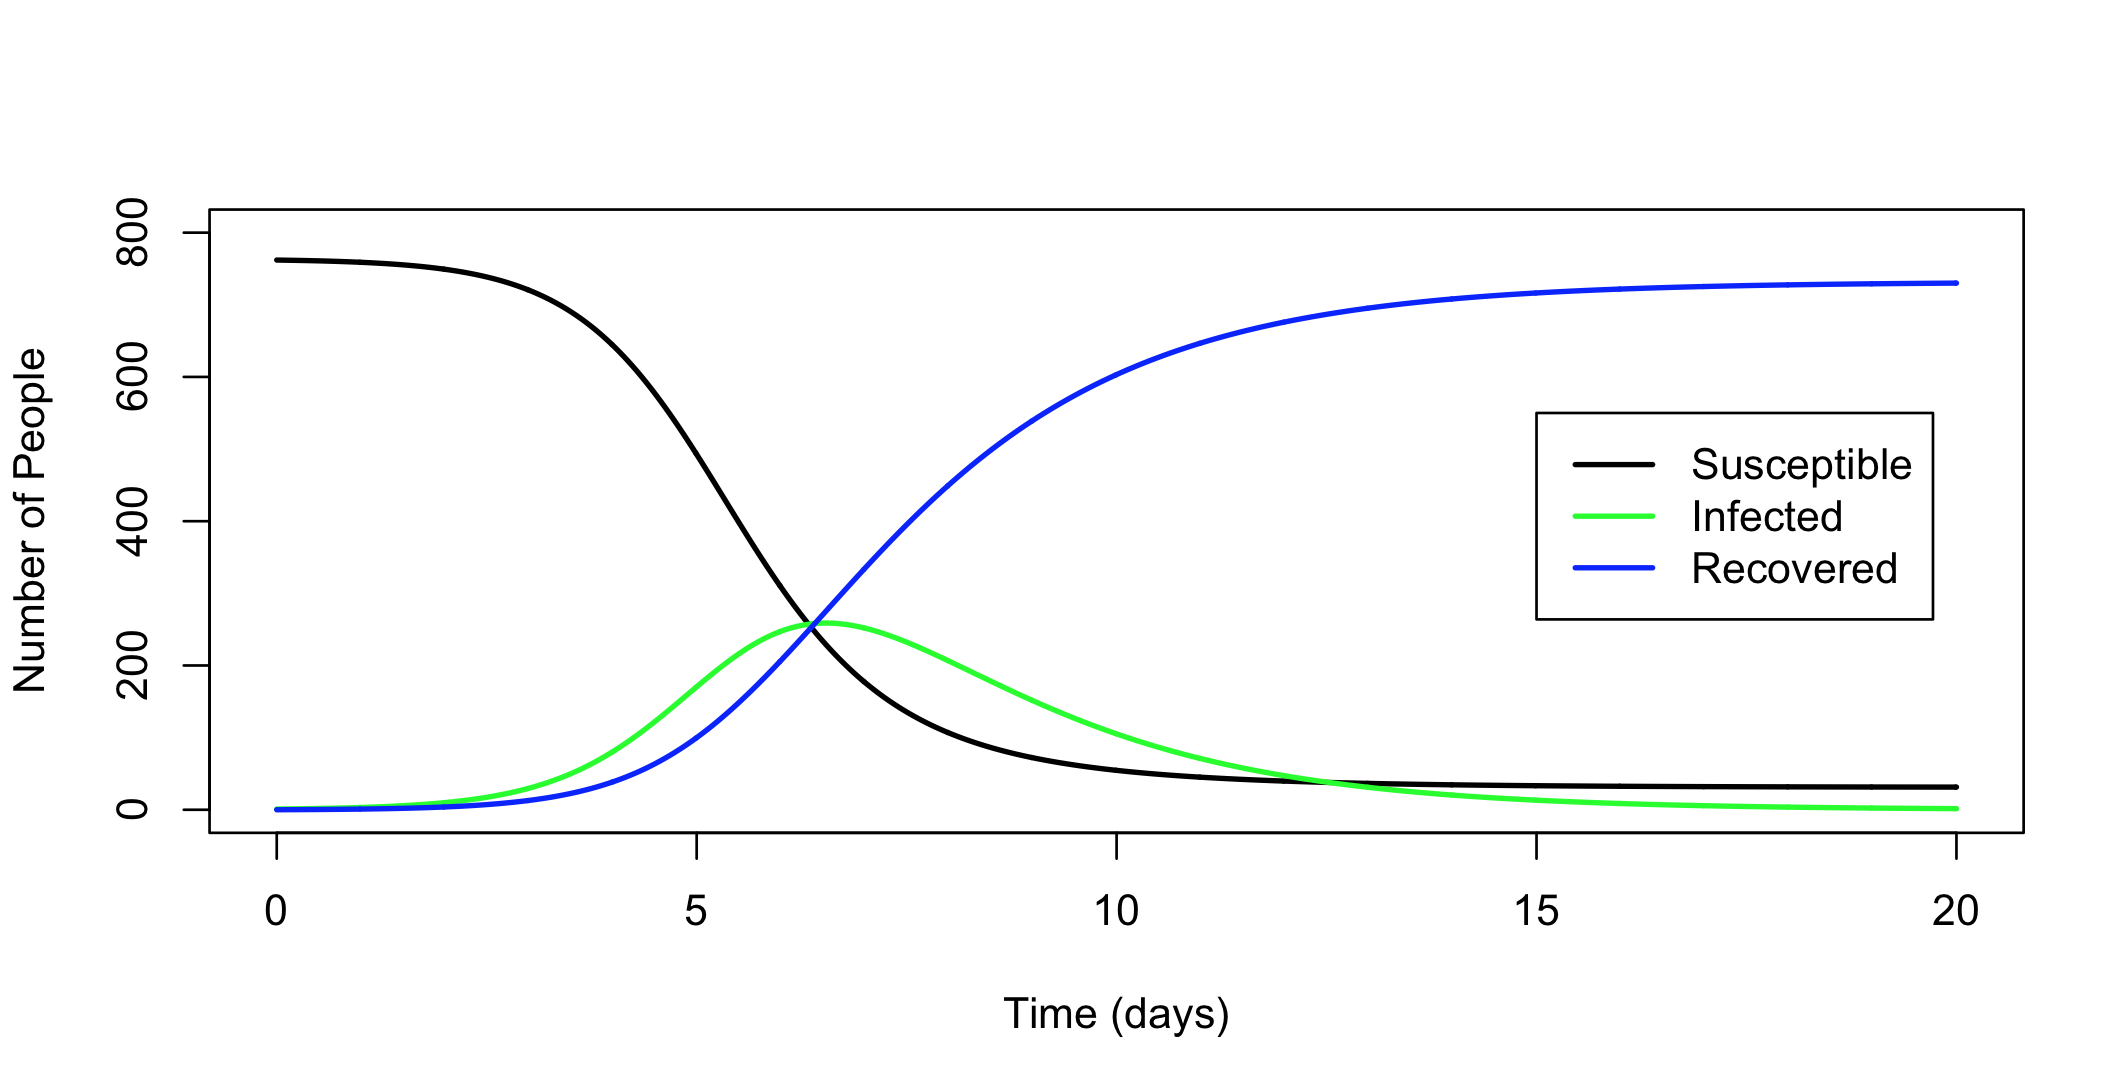
\includegraphics[width=\textwidth,height=\textheight,keepaspectratio]{sir.png}

        This plot shows the number of susceptibles slowly going down as people start to get infected. In the beginning you can see quite clearly how as the number of susceptibles goes down, the number of infected people goes up. The number of infected people however doesn't end up getting too high since people start to recover soon after they become infected. You can see that a short time after of susceptibles go down, the number recovered go up.
        \\
        \\
        Something interesting that I have found from looking at the graph is that when the amount of infected people hits 0, there are still susceptibles left and there are also still people who have not recovered (who aren't immune). This is because although the sickness hits the majority of people (in this case), there comes a stage where there are so many people that are immune that the disease can't really spread anymore. So in the end, some people stay susceptible however it doesn't matter since the disease has been eradicated.
    \subsection{Increasing the Initial Amount of Infected}
        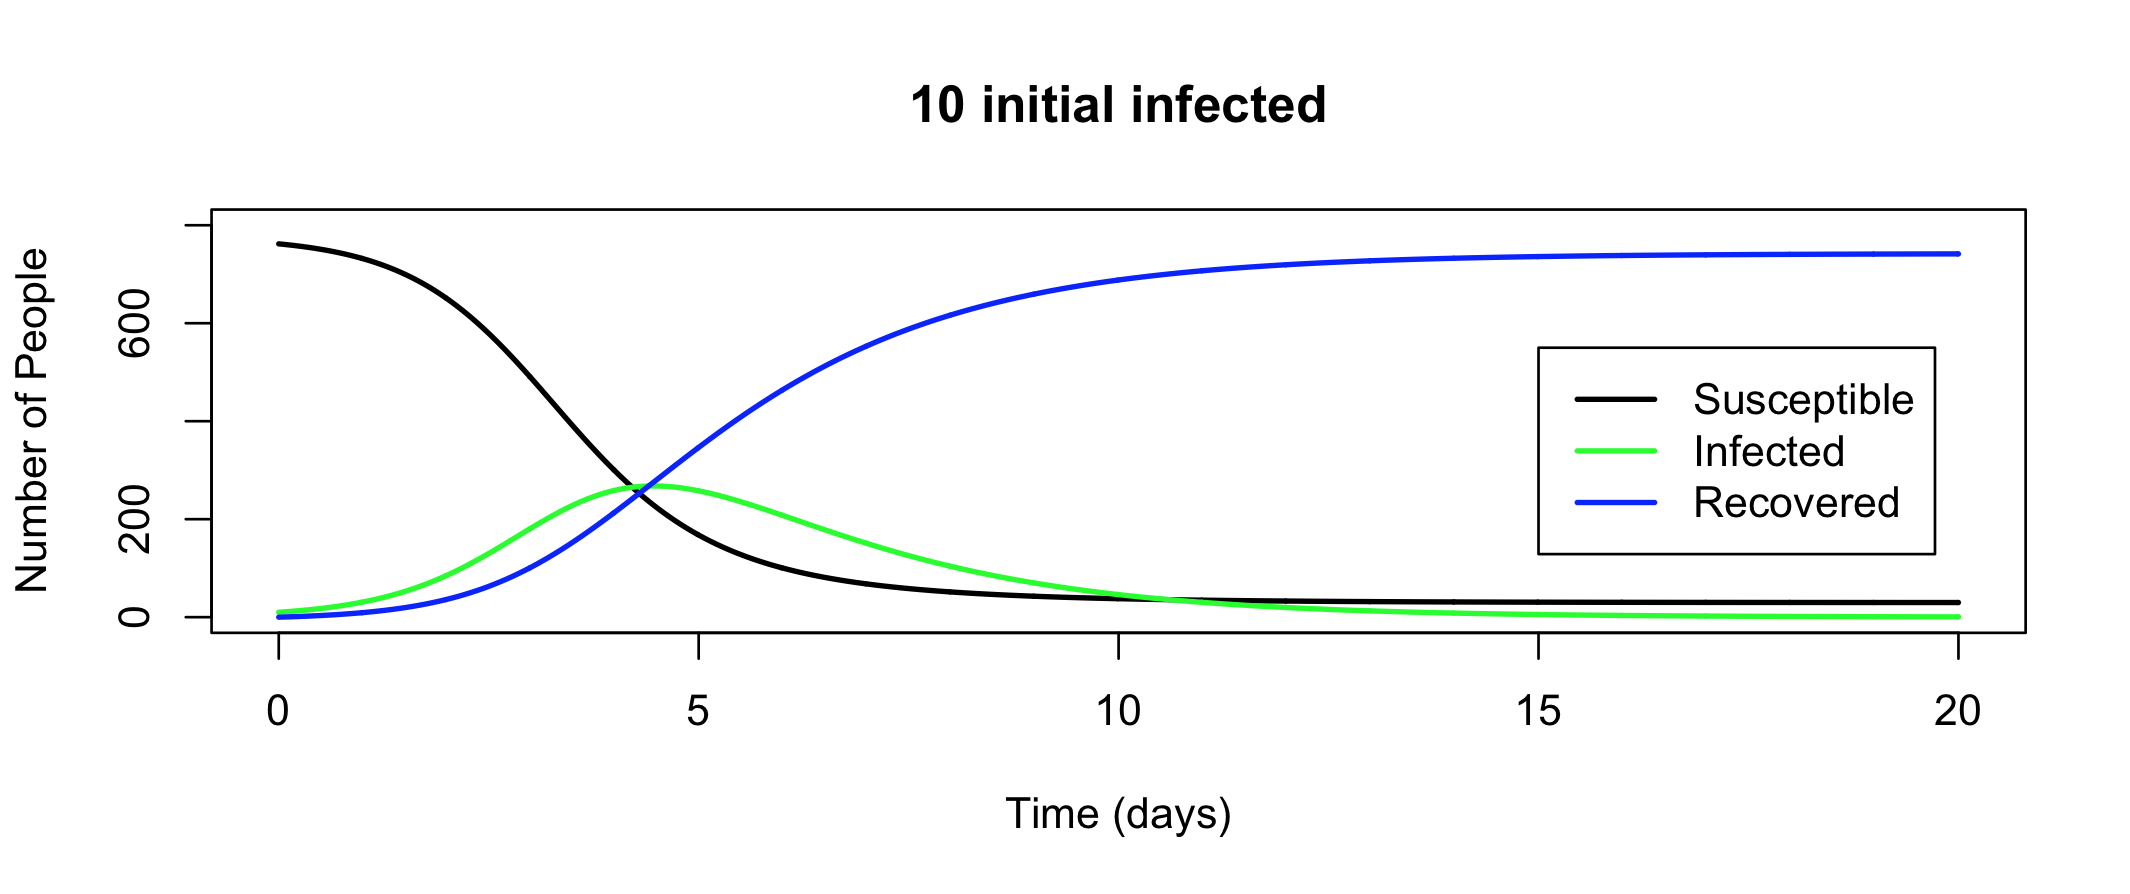
\includegraphics[width=\textwidth,height=\textheight,keepaspectratio]{sir_initial_infected_10.png}
        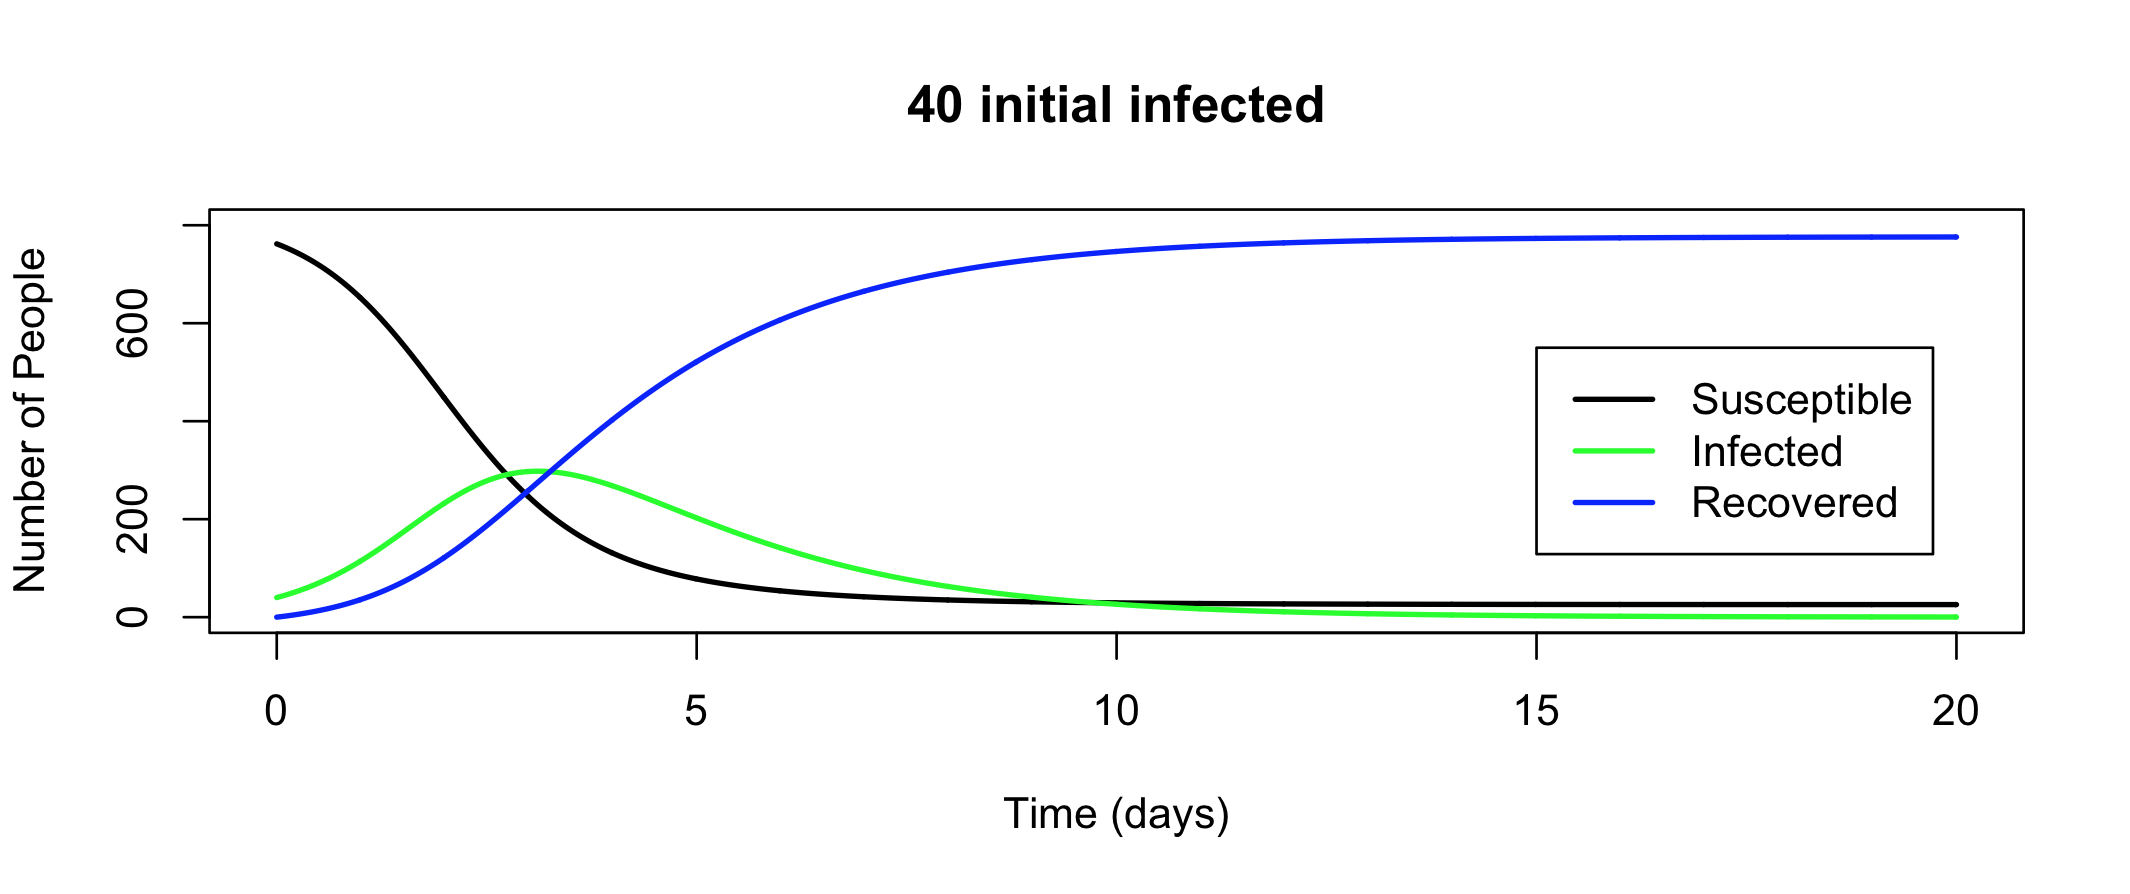
\includegraphics[width=\textwidth,height=\textheight,keepaspectratio]{sir_initial_infected_40.png}

        As you can see by the graphs above, changing the amount of people that were initially infected doesn't make a big difference in what actually happens. the only thing it does is increase the speed at which people get immunised (recovered). If the goal is to immunise as many people as quickly as possible it would make sense to get them infected as soon as possible. This is what happens when parents send their children to play with a child with chicken pox. They want to immunise the child as soon as possible (generally before they become an adult).
    
    \subsection{Increasing the Population}
        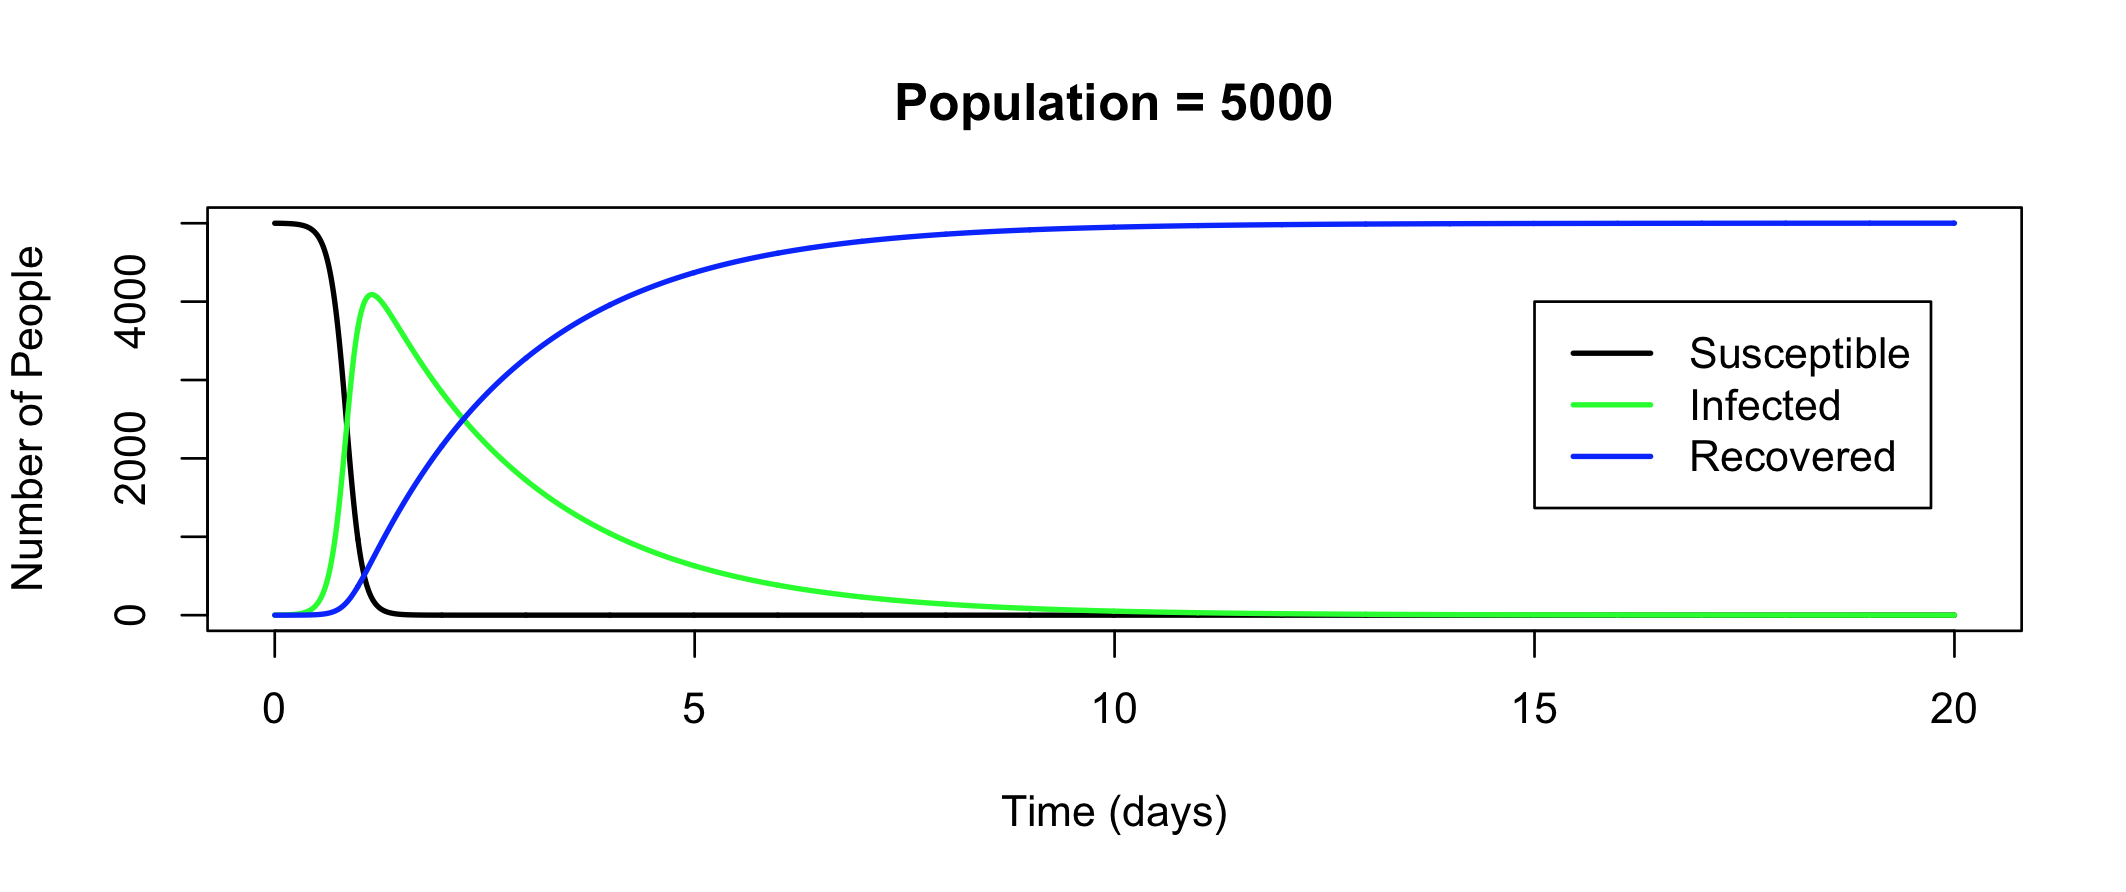
\includegraphics[width=\textwidth,height=\textheight,keepaspectratio]{sir_population_5000.png}
        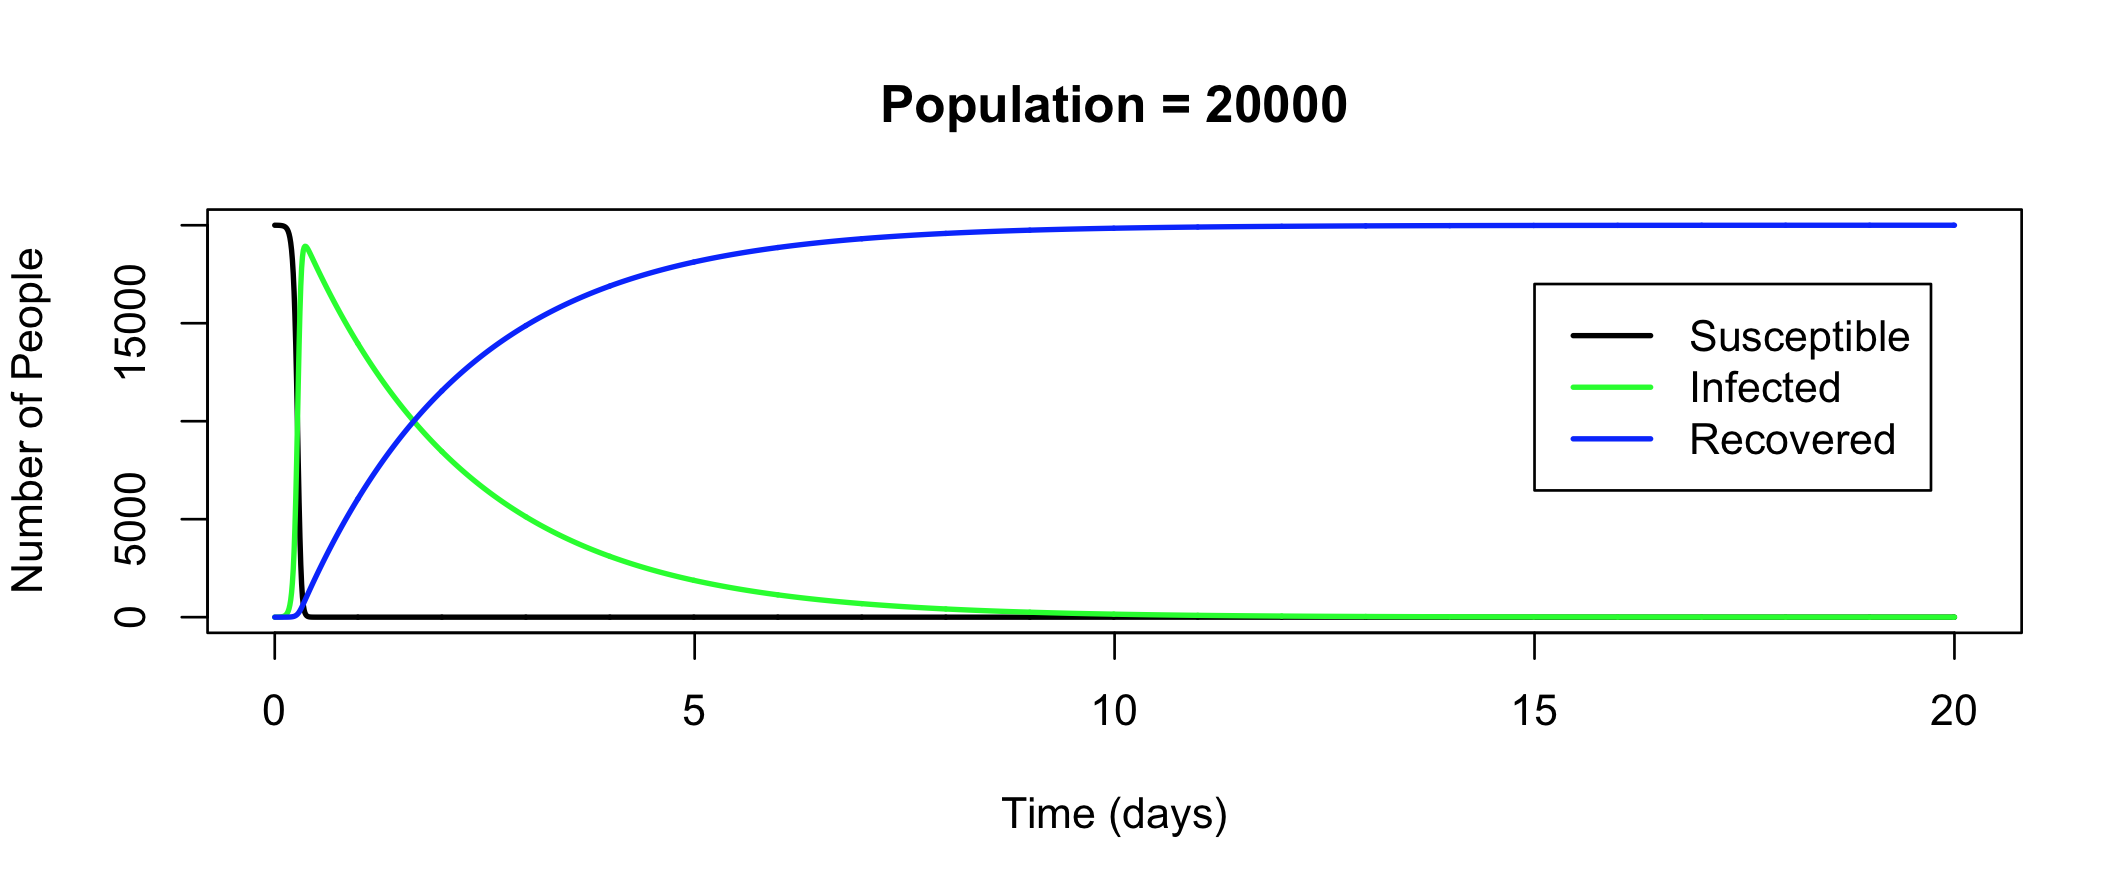
\includegraphics[width=\textwidth,height=\textheight,keepaspectratio]{sir_population_20000.png}

        By looking at the graphs, we can see that diseases spread much quicker when there is a larger population. It is also important to note that a larger percentage of the population becomes infected when there is a larger population. This is why people often seclude themselves when they become sick. Not exposing themselves to the large population of their co-workers and friends will reduce not only the amount of people that will get sick. It will also reduce the percentage of the people that you do encounter getting sick.

    \subsection{Increasing the Amount of Immunised People}
        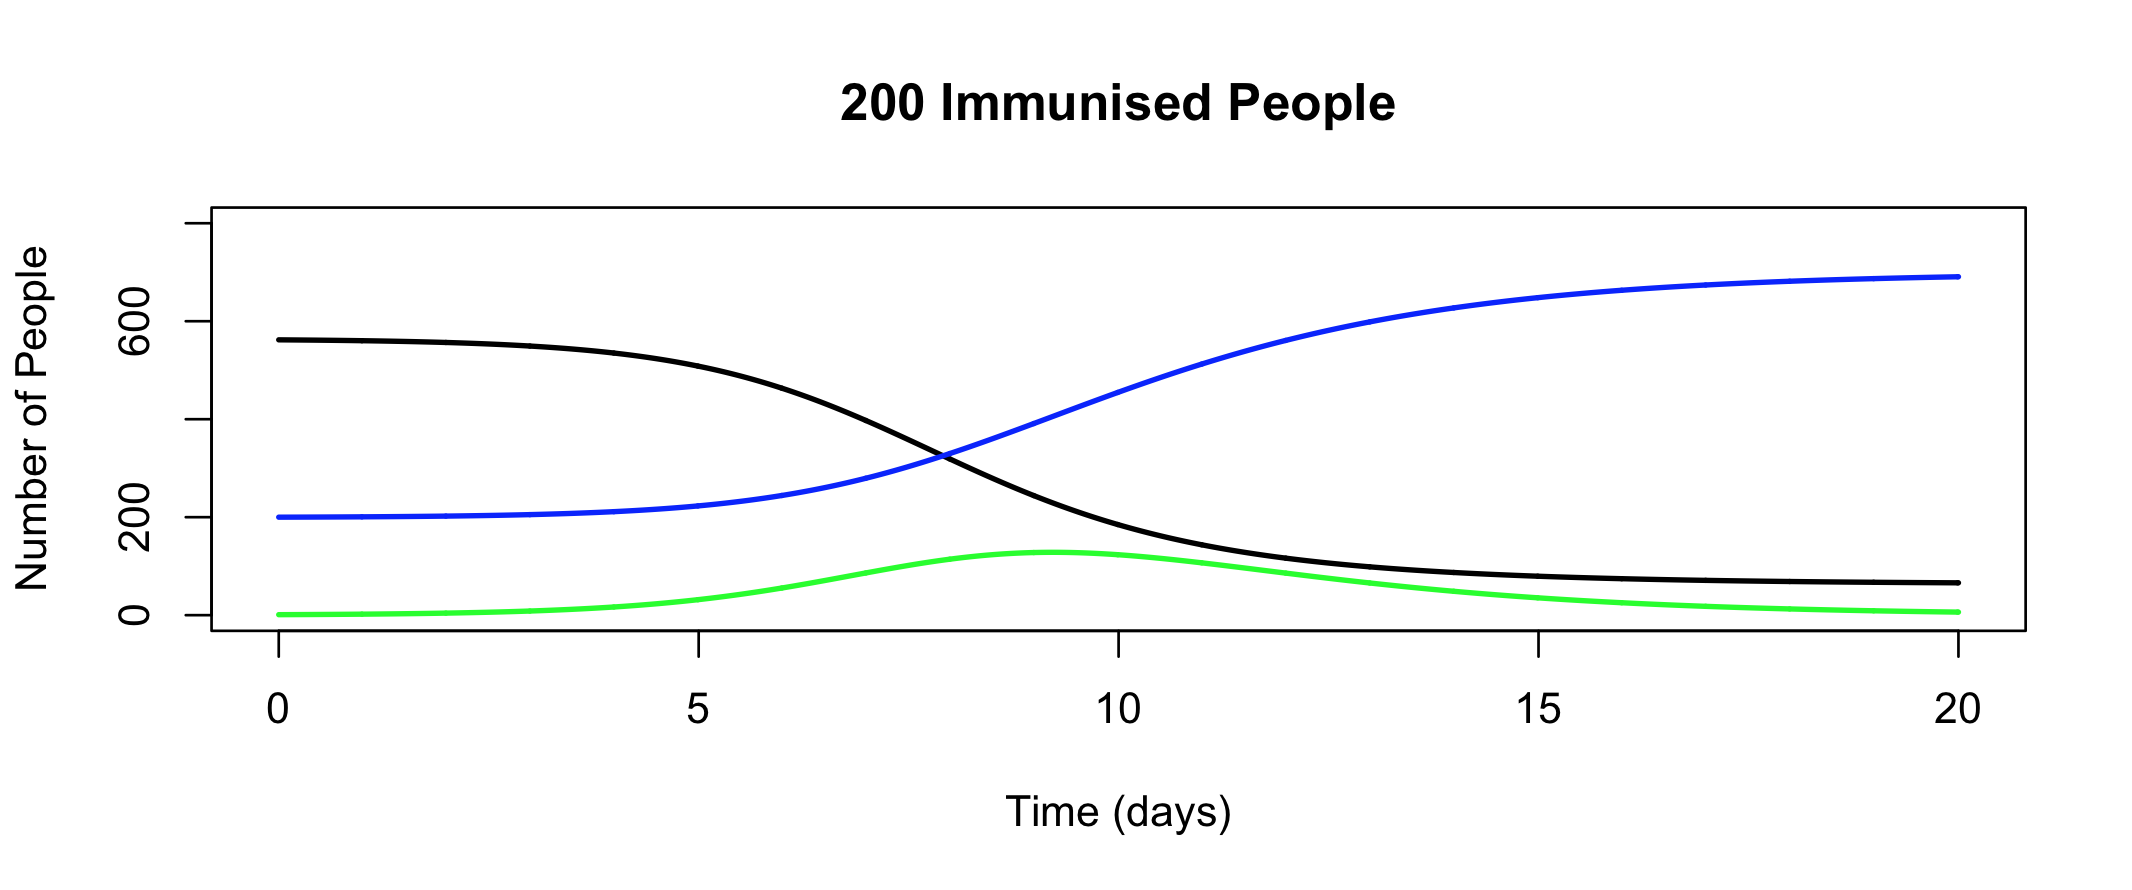
\includegraphics[width=\textwidth,height=\textheight,keepaspectratio]{sir_immunised_200.png}
        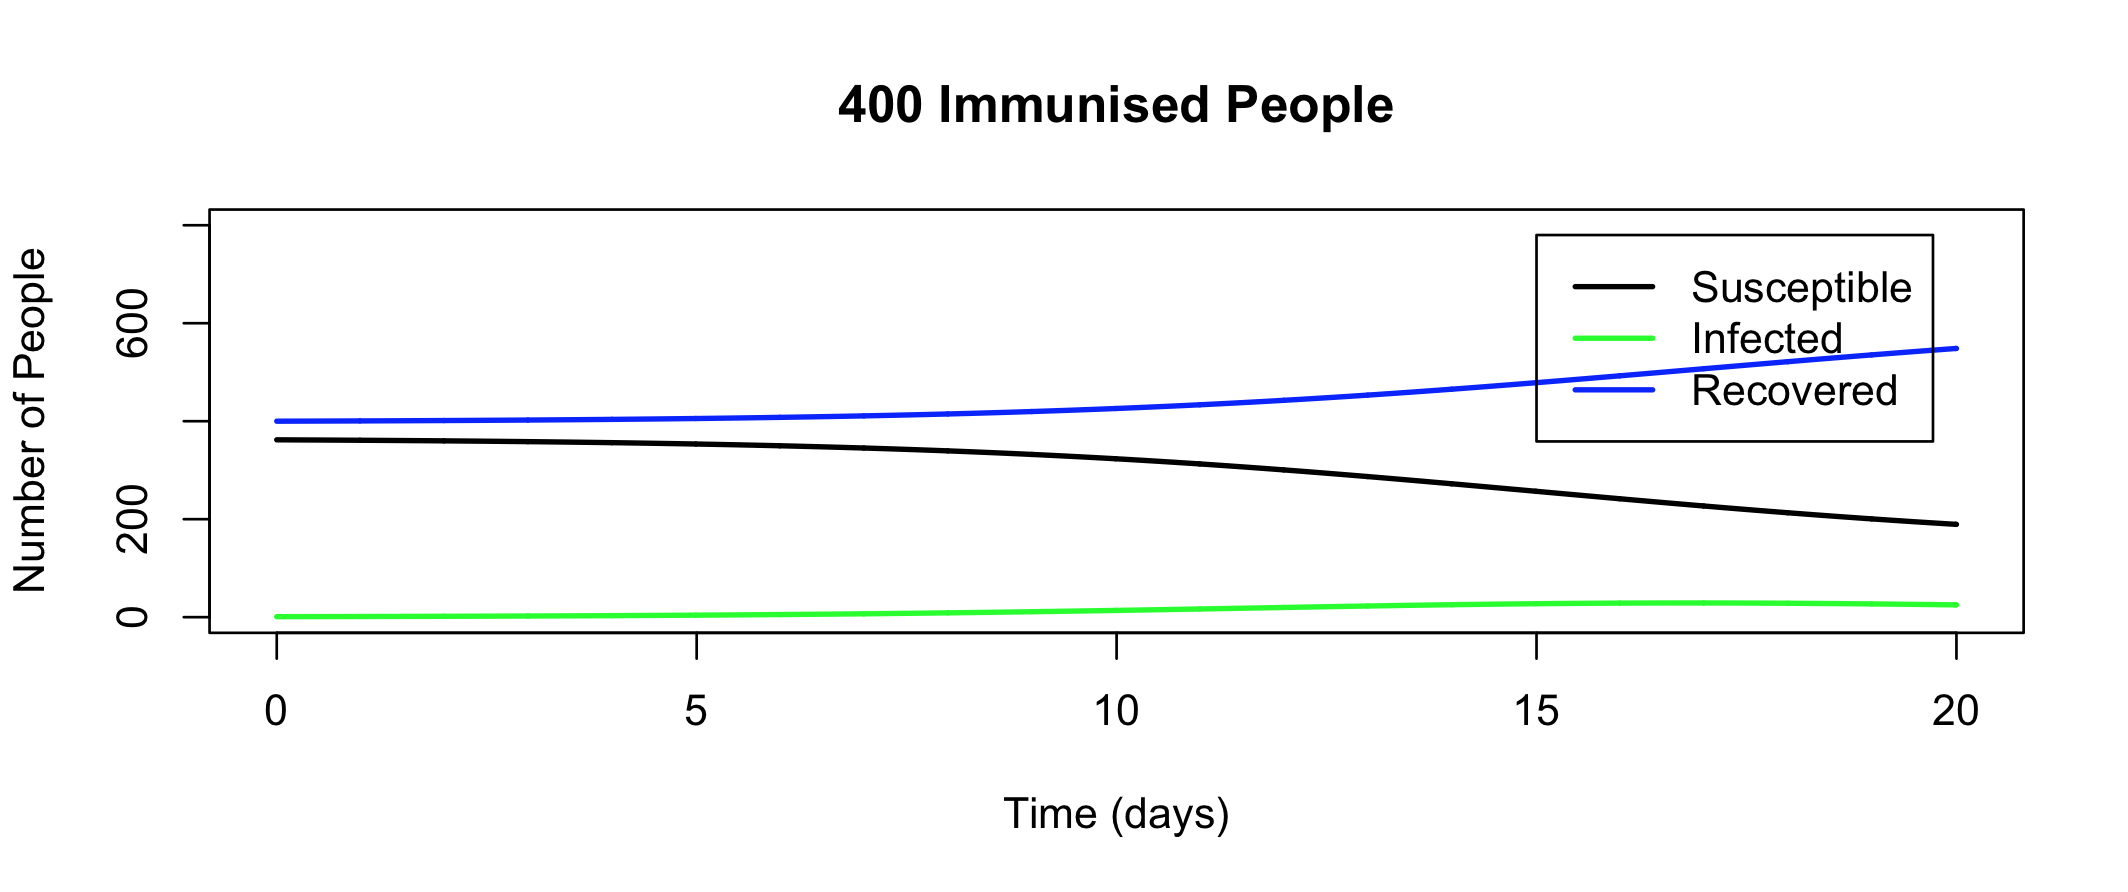
\includegraphics[width=\textwidth,height=\textheight,keepaspectratio]{sir_immunised_400.png}

        By Increasing the amount of immunised (recovered) people, we can see that the number of people who get infected goes down quite drastically. When just over half of the population was immunised, the disease infected barely anyone. This is why so many people are pushing for immunisation, because it makes a huge difference in the amount of people that get effected.

    \subsection{Increasing the Infection Rate}
        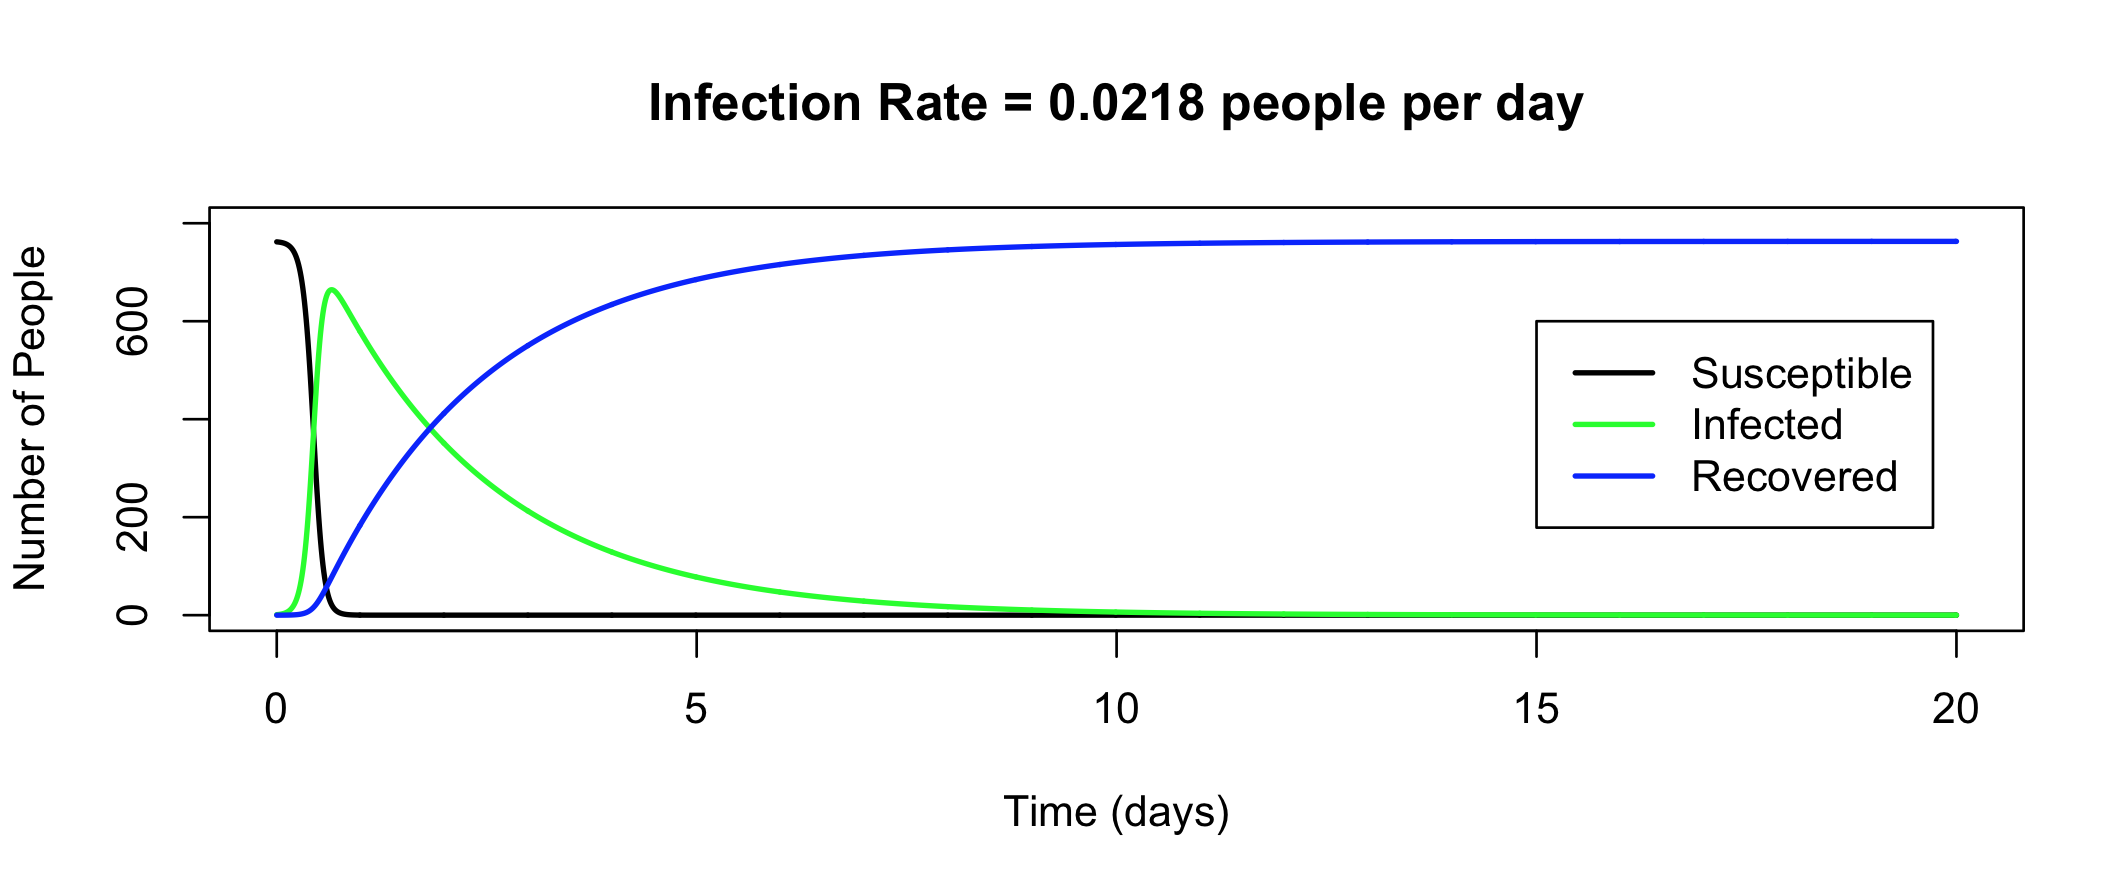
\includegraphics[width=\textwidth,height=\textheight,keepaspectratio]{sir_infection_00218.png}
        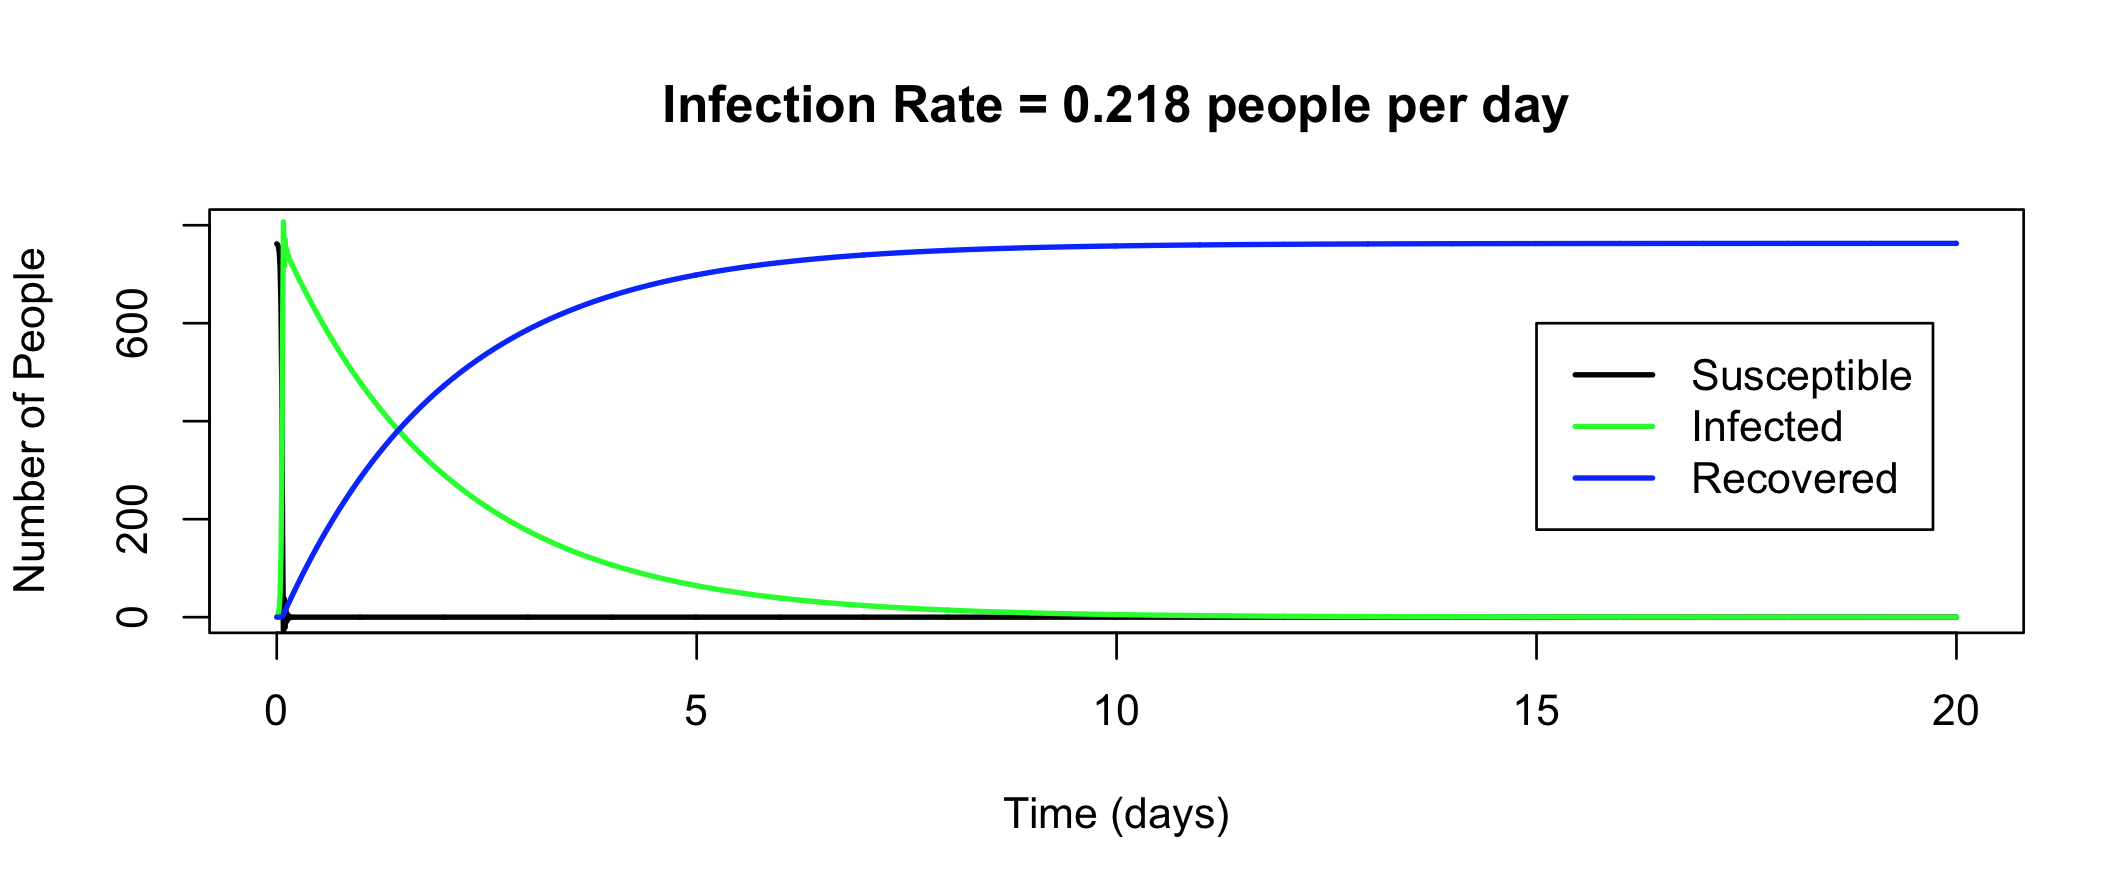
\includegraphics[width=\textwidth,height=\textheight,keepaspectratio]{sir_infection_0218.png}

        Increasing the infection rate does exactly what you would expect. It increases how quickly people get infected and therefore decreases the time it takes for the disease to die out. It also increases how many people actually get infected until the infection rate is so high that everyone gets infected.

    \subsection{Increasing the Recovery Rate}
        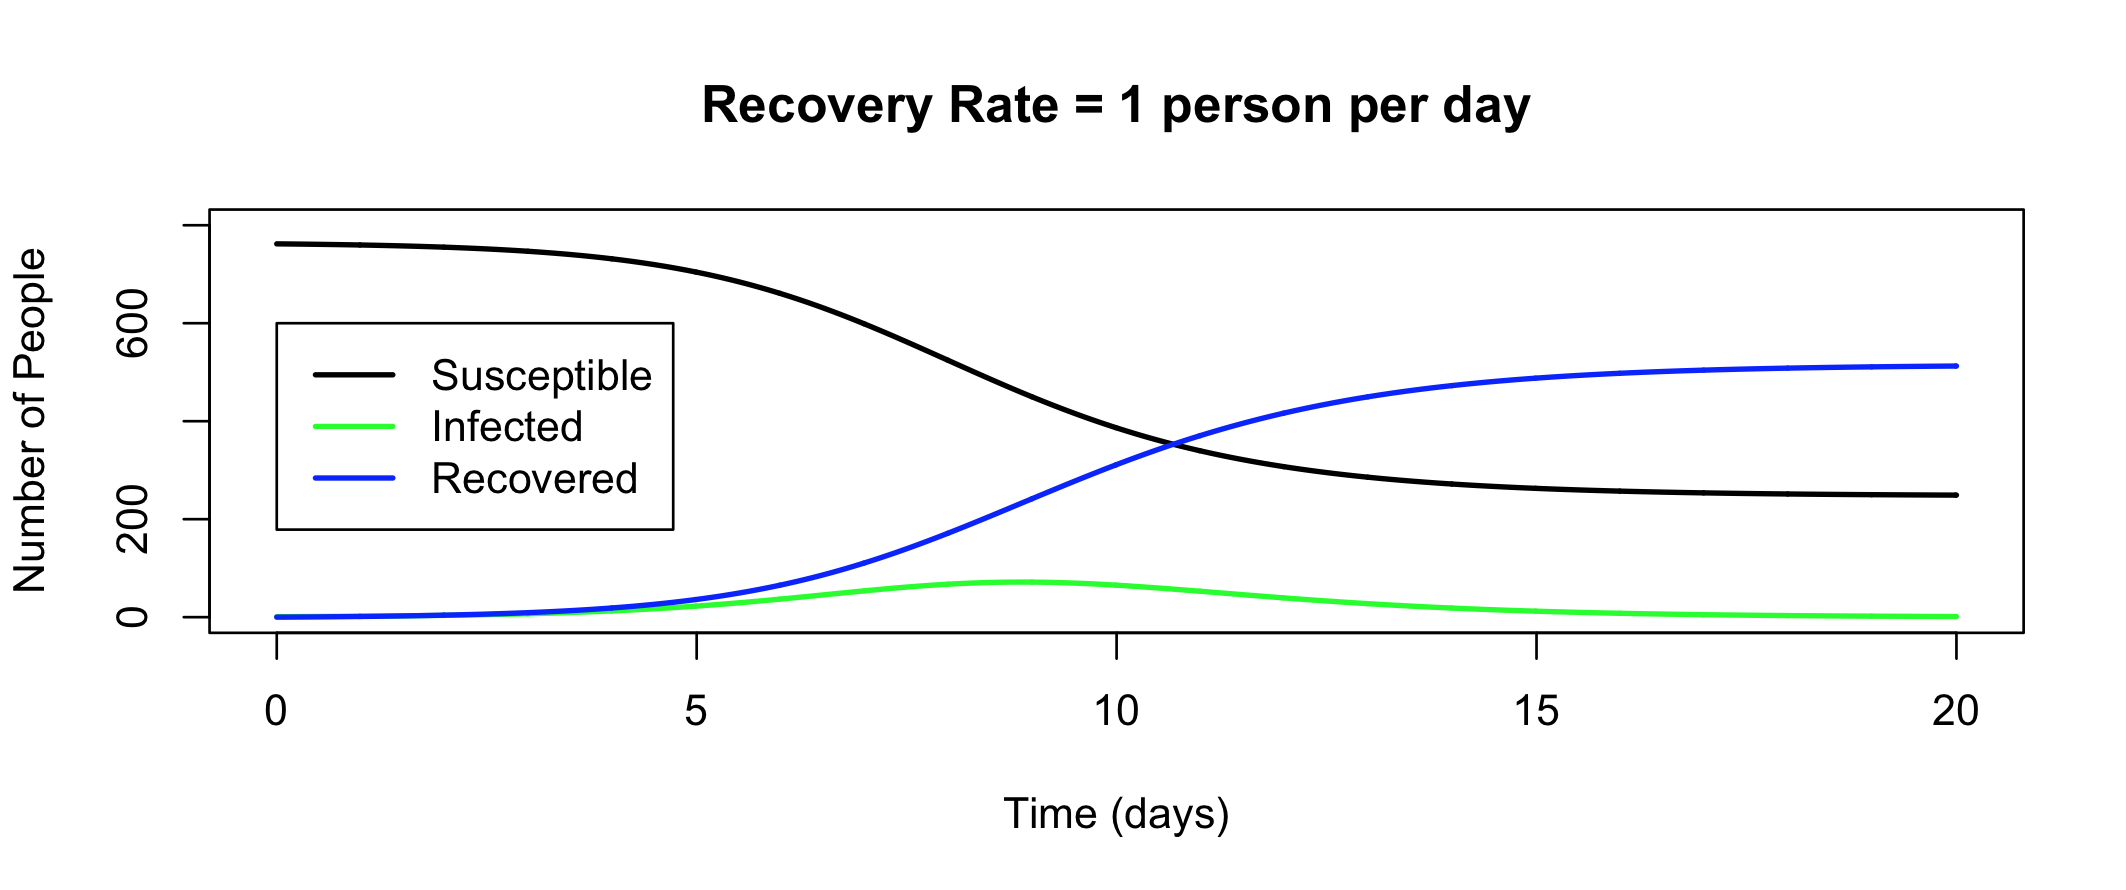
\includegraphics[width=\textwidth,height=\textheight,keepaspectratio]{sir_recovery_1.png}
        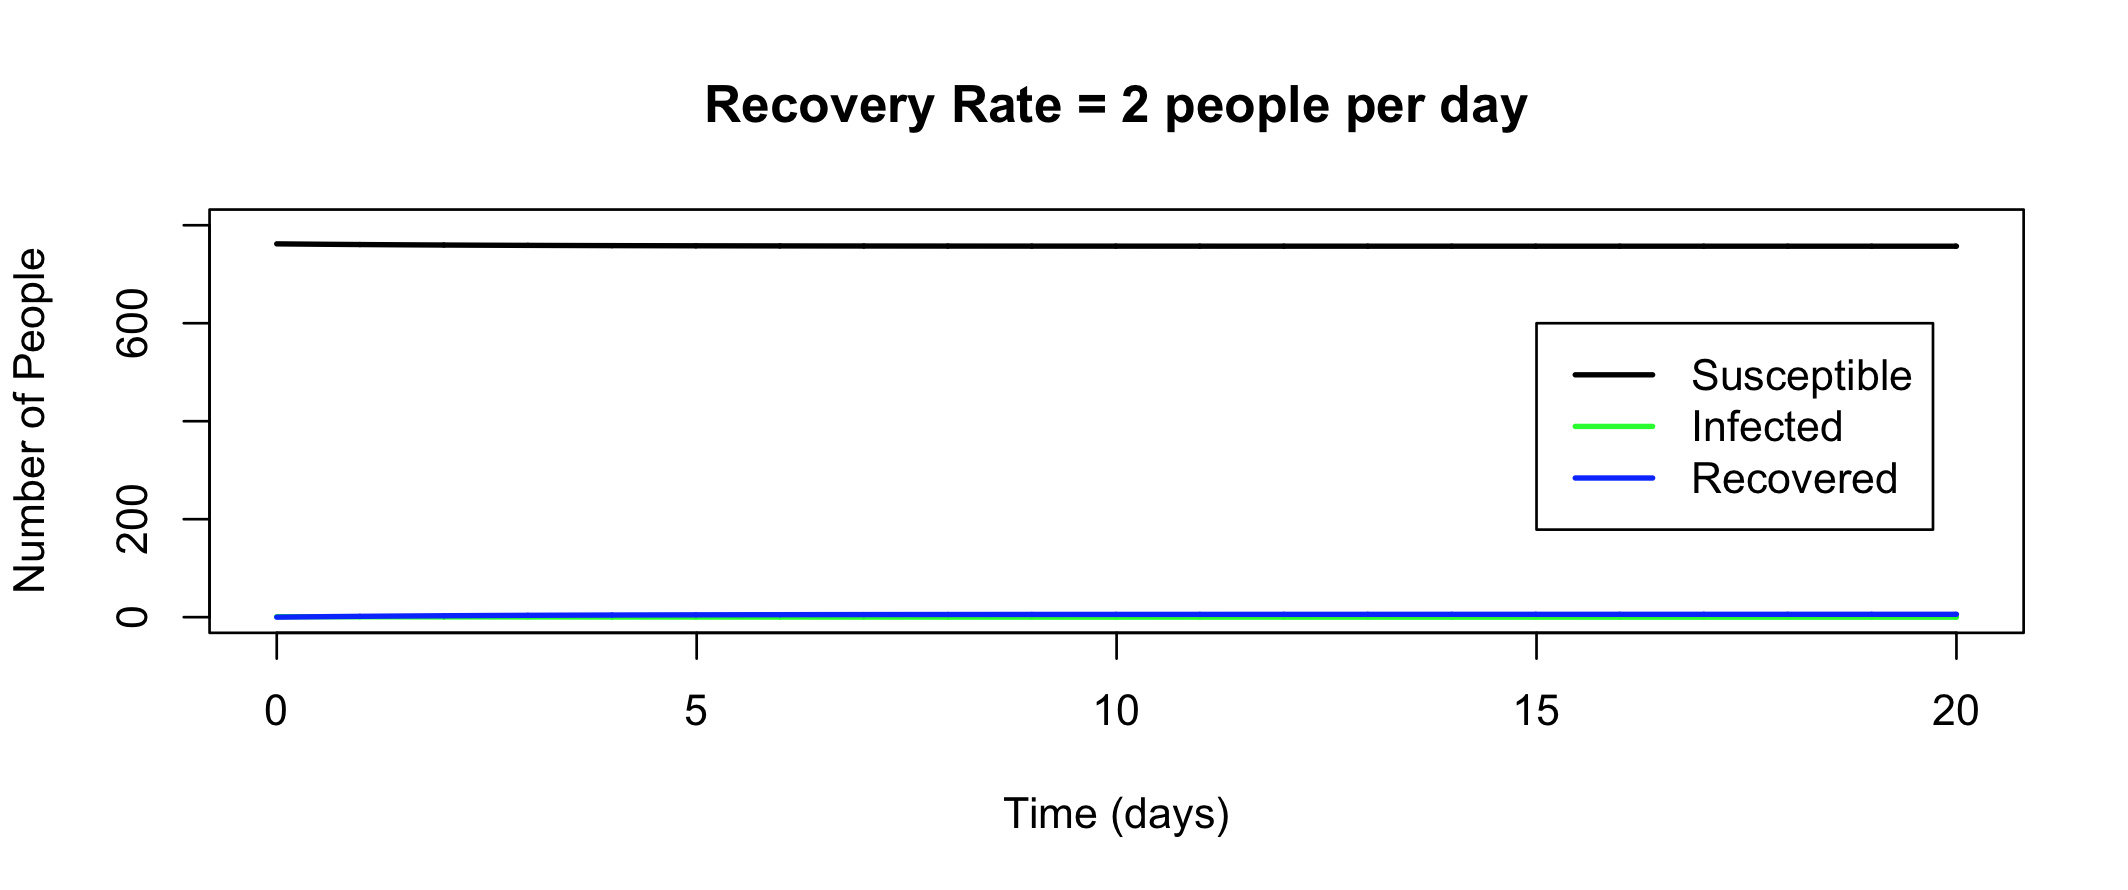
\includegraphics[width=\textwidth,height=\textheight,keepaspectratio]{sir_recovery_2.png}

        Changing the recovery rate does the opposite of what increasing the infection rate does. It reduces the amount of people that get sick however it increases the time it takes for the disease to die out. When the recovery rate gets too high, no-one ends up being effected since the person who has the disease recovers before the disease had the chance to spread.

    \subsection{Changing the Time Interval}
        After noticing how drastically the results change when the time interval changes, I decided to write a program to graph the difference in accuracy for different time interval sizes. This will also help in finding the time interval needed to get an accurate enough approximation without wasting unneeded computing resources. The graphs generated by the program are shown below.

        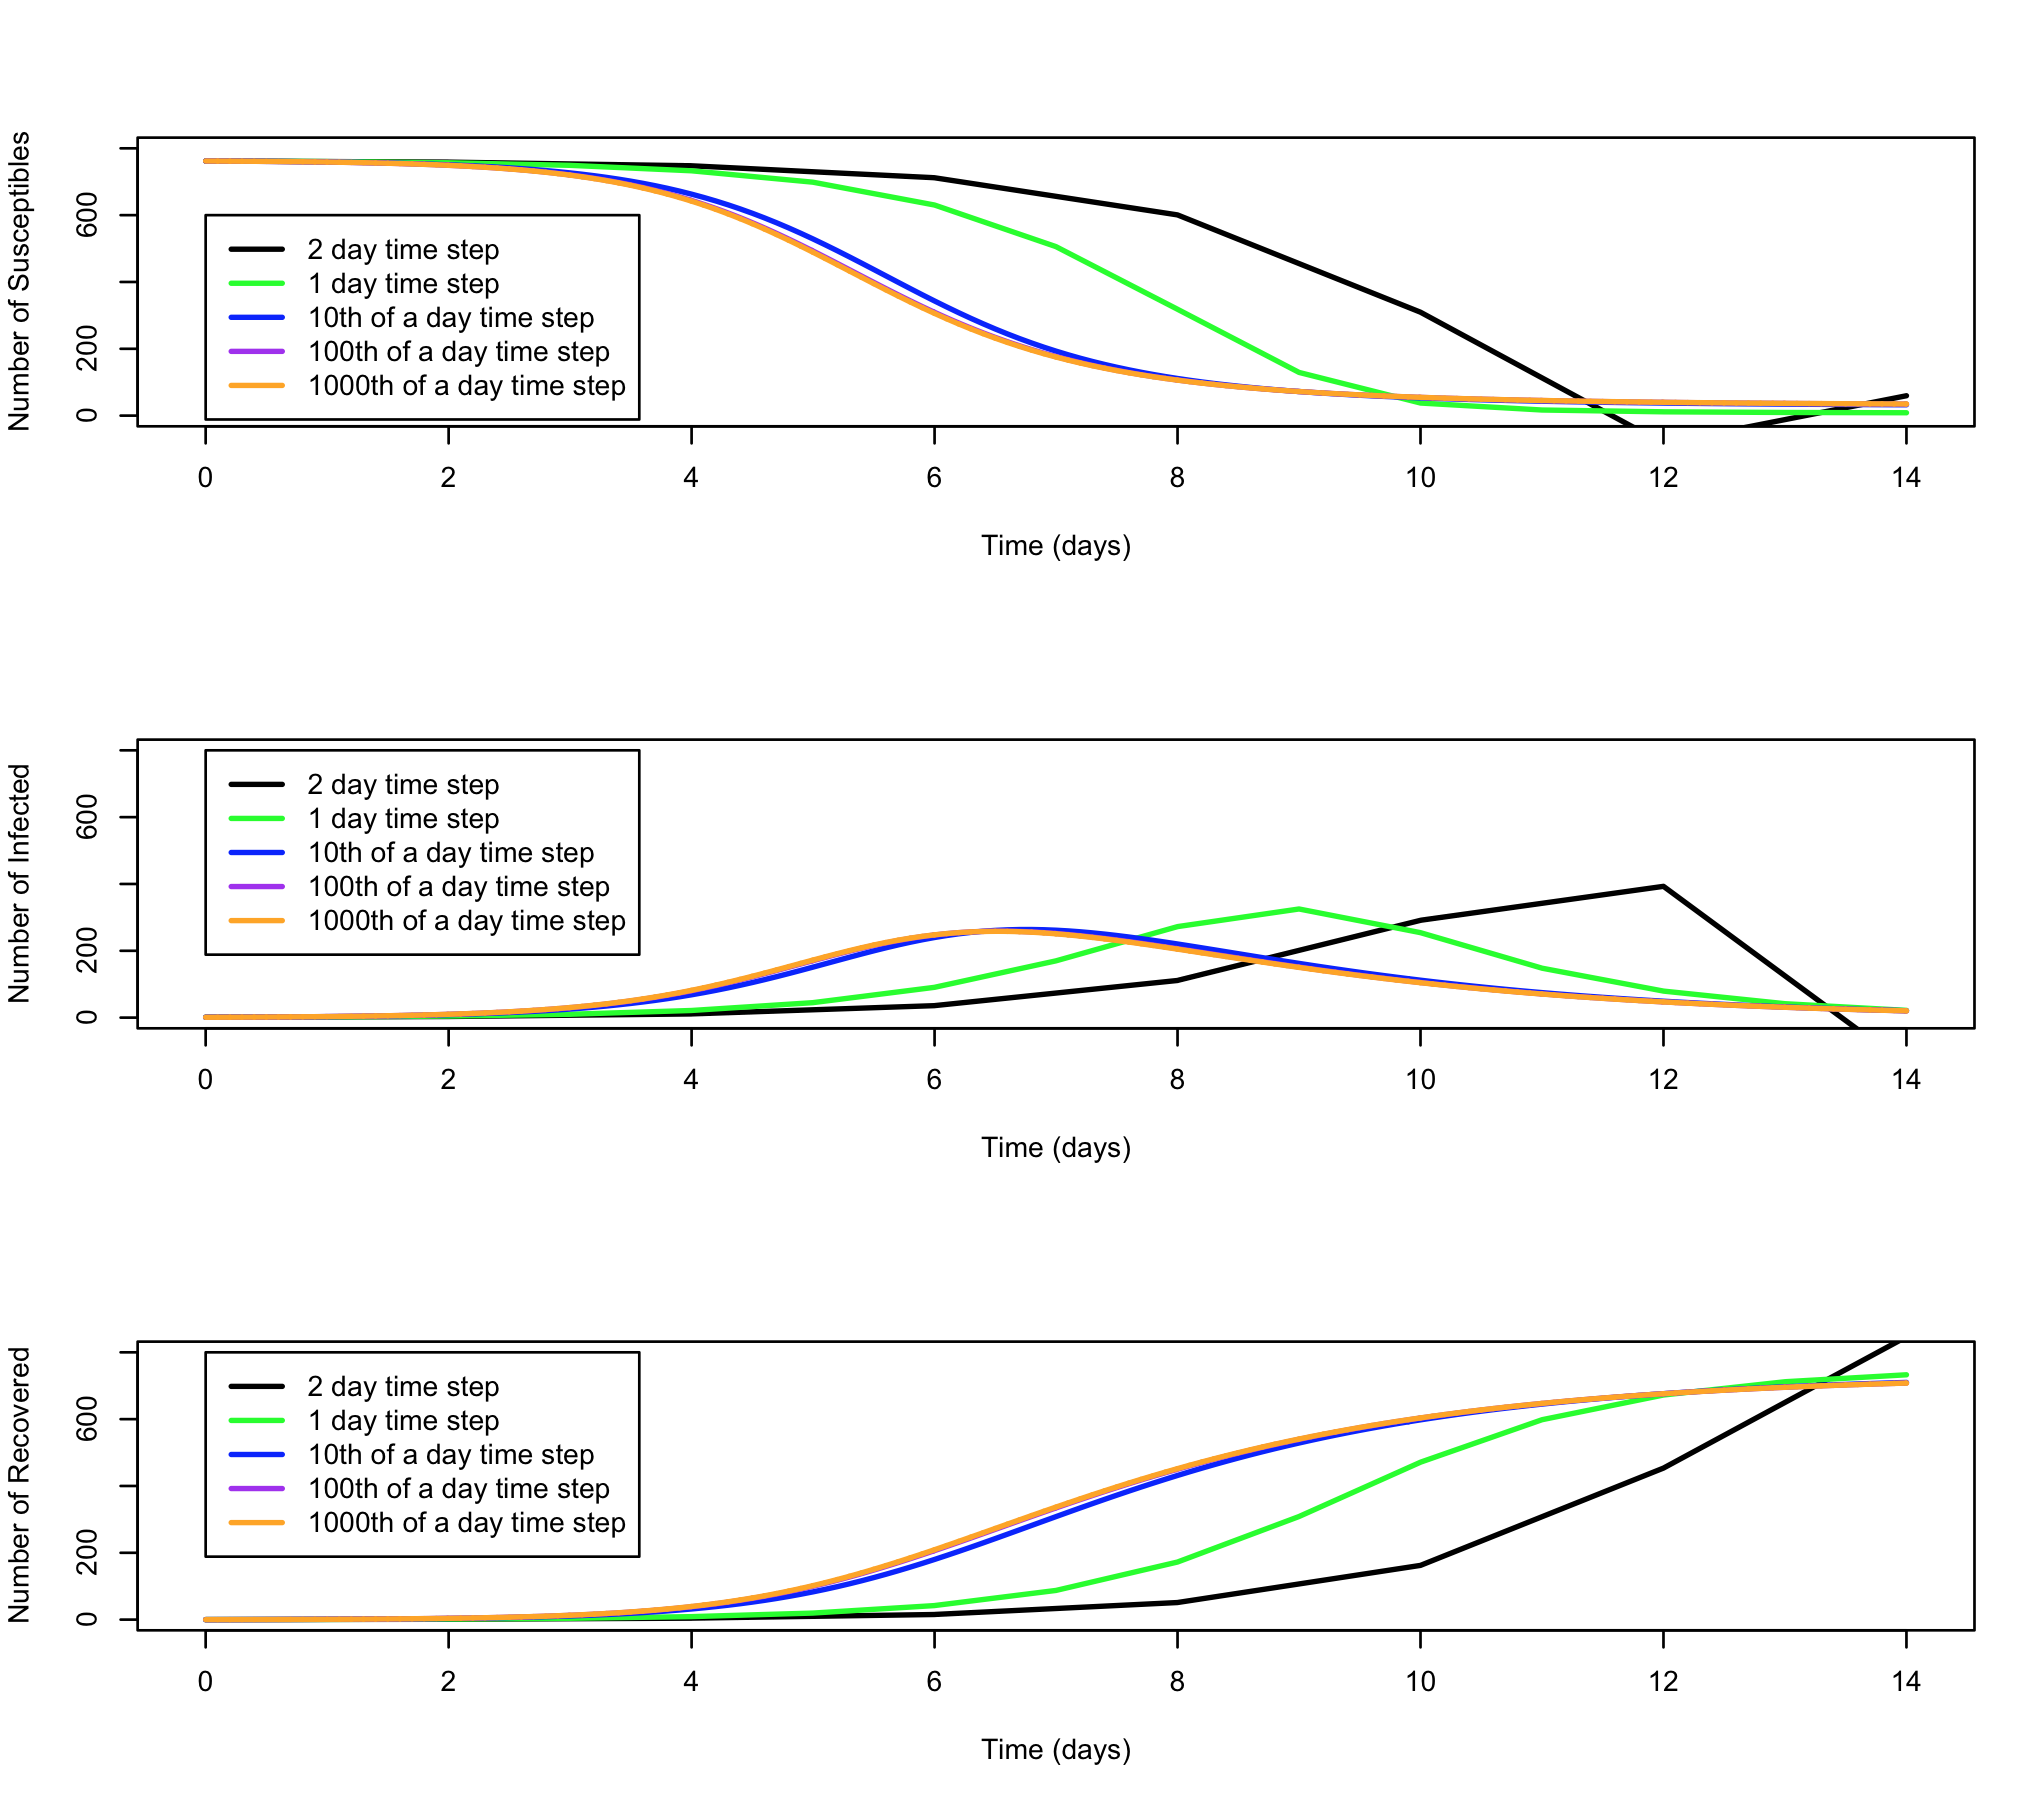
\includegraphics[width=\textwidth,height=\textheight,keepaspectratio]{time_interval_comparison.png}

        When we do calculations at more time steps in our graphs, we will get a more accurate result. From the graphs above, you can clearly see that there is quite a big difference in in the results obtained when we change the time steps. This drastic change is shown in all three graphs 
        \\
        \\
        At a time step of 2 days, the approximations actually get so bad that we calculate the number of susceptibles going below 0 (which obviously isn't possible). At a time step of 1 day we can see the shape of the graph, the way that we would expect it. However the time at which a certain amount of people are susceptible/infected/recovered is off by quite a margin.
        \\
        \\
        Going to a time step of a 10th of a day you can see, that there is a big change from the 1 day time step. We are starting to get a lot closer to the actual graph that we are supposed to see. In the pictures, you can't actually see the 100th of a day time step. This is because the 1000th of a day time step has been drawn (almost) directly over it. This is why I believe that the 100th of a day time step (recalculating every 0.01 days) is the best in terms of getting a very accurate approximation without expending an unnecessary amount of computations. It is still a bit better than the 10th of a day time step but going any further doesn't really give more information.

\section{Conclusion}
    Getting a disease or virus is never a pleasant thing so we alway want to minimise the affect on others when we have these. From the analysis done in this report, we can come to the conclusion that the best steps to preventing the spread of disease are keeping the population around you small and getting immunised. Both of these things will keep others from getting sick and immunisation as a bonus will also stop you from getting sick.

\end{document}